\section{Data generation}\label{sec:data}

\subsection{Sampling}
For each of the four cases (NMOS ON, NMOS OFF, PMOS ON, PMOS OFF), 10{,}000 samples were drawn. Every parameter is drawn independently;
$\Vdd$ is drawn first because the ranges of $V_d$ and $V_s$ depend on it (\cref{tab:sampling}). The five process parameters are drawn as the nominal
value of the model card multiplied by a factor uniform in $[0.9, 1.1]$, separately for NMOS and PMOS (so the PMOS threshold stays negative).
Gate and body voltages are fixed by the case.

\begin{table}[H]\centering\small
\begin{tabular}{ll}
\toprule
Parameter & Distribution\\
\midrule
$\Vdd$ & uniform, $1\,\mathrm{V}\pm10\,\%$\\
$V_d$, $V_s$ & uniform, $0$ to $\Vdd$\\
$W$ & uniform, $1\times\Lmin$ to $8\times\Lmin$ ($22$--$176\,\mathrm{nm}$)\\
Temperature & uniform, $-40$ to $125\,^\circ$C\\
\texttt{vth0}, \texttt{toxe}, \texttt{ndep}, \texttt{u0}, \texttt{xj} & uniform, nominal value of the card $\pm10\,\%$, separate NMOS/PMOS draws\\
$(V_g, V_b)$ & NMOS ON $(\Vdd,0)$, NMOS OFF $(0,0)$, PMOS ON $(0,\Vdd)$, PMOS OFF $(\Vdd,\Vdd)$\\
\bottomrule
\end{tabular}
\caption{Sampling distributions of the transistor datasets (assignment, Section 4).}\label{tab:sampling}
\end{table}

The random generator of each case is seeded with (base seed, case index, batch). A sample whose simulation fails would be replaced from a
deterministic extra batch so that every file has exactly 10{,}000 rows; no simulation failed. The four datasets
(\texttt{data/transistor/*.csv}, columns \texttt{vdd, temp, w, vd, vs, vg, vb, vth0, toxe, ndep, u0, xj, id, ig, is, ib}) took about two minutes
per case with parallel ngspice processes.

\subsection{Netlists}
Each sample is written as a self-contained single-transistor netlist (examples in \texttt{data/netlists/\allowbreak single\_transistor/}):
\begin{itemize}
  \item both model cards are inlined; the five sampled process values replace the nominal values in the card of the device under test;
  \item one MOSFET with $L=22\,\mathrm{nm}$, the sampled $W$ and $AD=AS=W\cdot L_{\mathrm{diff}}$;
  \item \textbf{one DC voltage source per terminal} ($V_d$, $V_g$, $V_s$, $V_b$), the sampled temperature (\texttt{.temp}) and the mandated
        \texttt{.options} line;
  \item an operating-point analysis that prints the four source currents with ten significant digits.
\end{itemize}
The terminal currents are the negated source currents, i.e.\ they are defined positive \emph{into} the device, so that $I_d+I_g+I_s+I_b=0$.

\subsection{Training, validation and test split}
Each 10{,}000-row dataset is split at random into 70\,\% training, 15\,\% validation and 15\,\% test rows (7{,}000 / 1{,}500 / 1{,}500) with a fixed
seed (\texttt{scripts/03\_make\_splits.py}, \texttt{data/splits/}). Model types, hyper-parameters and all design choices were selected on the validation
rows only; the test rows were used once, to report the final models.

\paragraph{Additional training data.} The assignment allows the number of samples to be increased. Two training-only sets were generated in the same way
(scripts \texttt{01b}, \texttt{01c}); the delivered 10{,}000-row datasets and the validation and test splits are unchanged:
\begin{itemize}
  \item \textbf{30{,}000 extra uniform rows per case} (\texttt{data/transistor\_extra/}), drawn from exactly the distributions of \cref{tab:sampling}.
        Rows 0--24{,}999 are added to the training set; rows 25{,}000--29{,}999 are a hold-out set that is never trained on.
  \item \textbf{20{,}000 rail-corner rows per case} (\texttt{data/transistor\_edge/}). $\Vdd$, temperature and process are drawn as above, but each of
        $V_d$ and $V_s$ is placed exactly at a rail (0 or $\Vdd$) with probability 40\,\%, within $0.1\,\Vdd\,u^2$ of a rail with probability 40\,\%
        and uniformly otherwise, and $W$ is drawn log-uniformly. In a logic gate every source and drain sits at, or within microvolts of, a rail,
        where uniform sampling places very few points. Only this a-priori fact is used---no gate or circuit SPICE result. Rows 0--15{,}999 are
        training rows, 16{,}000--17{,}999 join the validation set and 18{,}000--19{,}999 are a rail-corner hold-out.
\end{itemize}
In total 120{,}000 transistor simulations were run; none failed.

\subsection{Data check}
\paragraph{Kirchhoff check.} \Cref{tab:kirchhoff} gives the residual $|I_d+I_g+I_s+I_b|$ of every sample. For NMOS ON, NMOS OFF and PMOS ON the median
relative residual is about $10^{-10}$, i.e.\ the netlists conserve current to the printed precision. The larger \emph{relative} residuals---the PMOS
OFF case and the tail of NMOS ON---occur in samples whose currents are themselves at the numerical floor (29\,\% of the PMOS OFF rows have no current
above $10^{-16}$\,A); the \emph{absolute} residual never exceeds $5\times10^{-14}$\,A and is below $2\times10^{-15}$\,A for both OFF cases.
\begin{table}[H]
\centering
{\small
\begin{adjustbox}{max width=\linewidth}
\begin{tabular}{lrrrrr}
\toprule
case & abs. median [A] & abs. P95 [A] & abs. max [A] & rel. median & rel. P95 \\
\midrule
NMOS ON & $2.72\times10^{-16}$ & $4.12\times10^{-15}$ & $5.14\times10^{-14}$ & $2.55\times10^{-10}$ & $2.31\times10^{-4}$ \\
NMOS OFF & $1.76\times10^{-25}$ & $2.51\times10^{-22}$ & $5.39\times10^{-21}$ & $5.68\times10^{-11}$ & $2.62\times10^{-10}$ \\
PMOS ON & $6.84\times10^{-17}$ & $3.55\times10^{-15}$ & $4.43\times10^{-14}$ & $1.84\times10^{-10}$ & $8.73\times10^{-5}$ \\
PMOS OFF & $3.30\times10^{-17}$ & $3.19\times10^{-16}$ & $1.80\times10^{-15}$ & $1.19\times10^{-3}$ & $9.34\times10^{-1}$ \\
\bottomrule
\end{tabular}
\end{adjustbox}
}
\caption{Kirchhoff check on the four 10{,}000-row datasets: residual $|I_d+I_g+I_s+I_b|$ per sample, absolute and relative to the largest terminal current of the sample (relative values for samples whose largest current exceeds $10^{-16}$\,A).}
\label{tab:kirchhoff}
\end{table}



\paragraph{Numerical noise floor.} The current distributions (\cref{fig:dist}) show that not every value is physical signal. The gate current of
the OFF devices, for example, is never above $10^{-15}$\,A and otherwise takes a few discrete values that are multiples of a double-precision
rounding step; tighter solver tolerances reproduce the same values. Currents below $\Ifl=10^{-15}$\,A are therefore treated as the noise floor of
the reference: they cannot be learned and are not scored (\cref{sec:metrics}).

\begin{figure}[!htbp]\centering
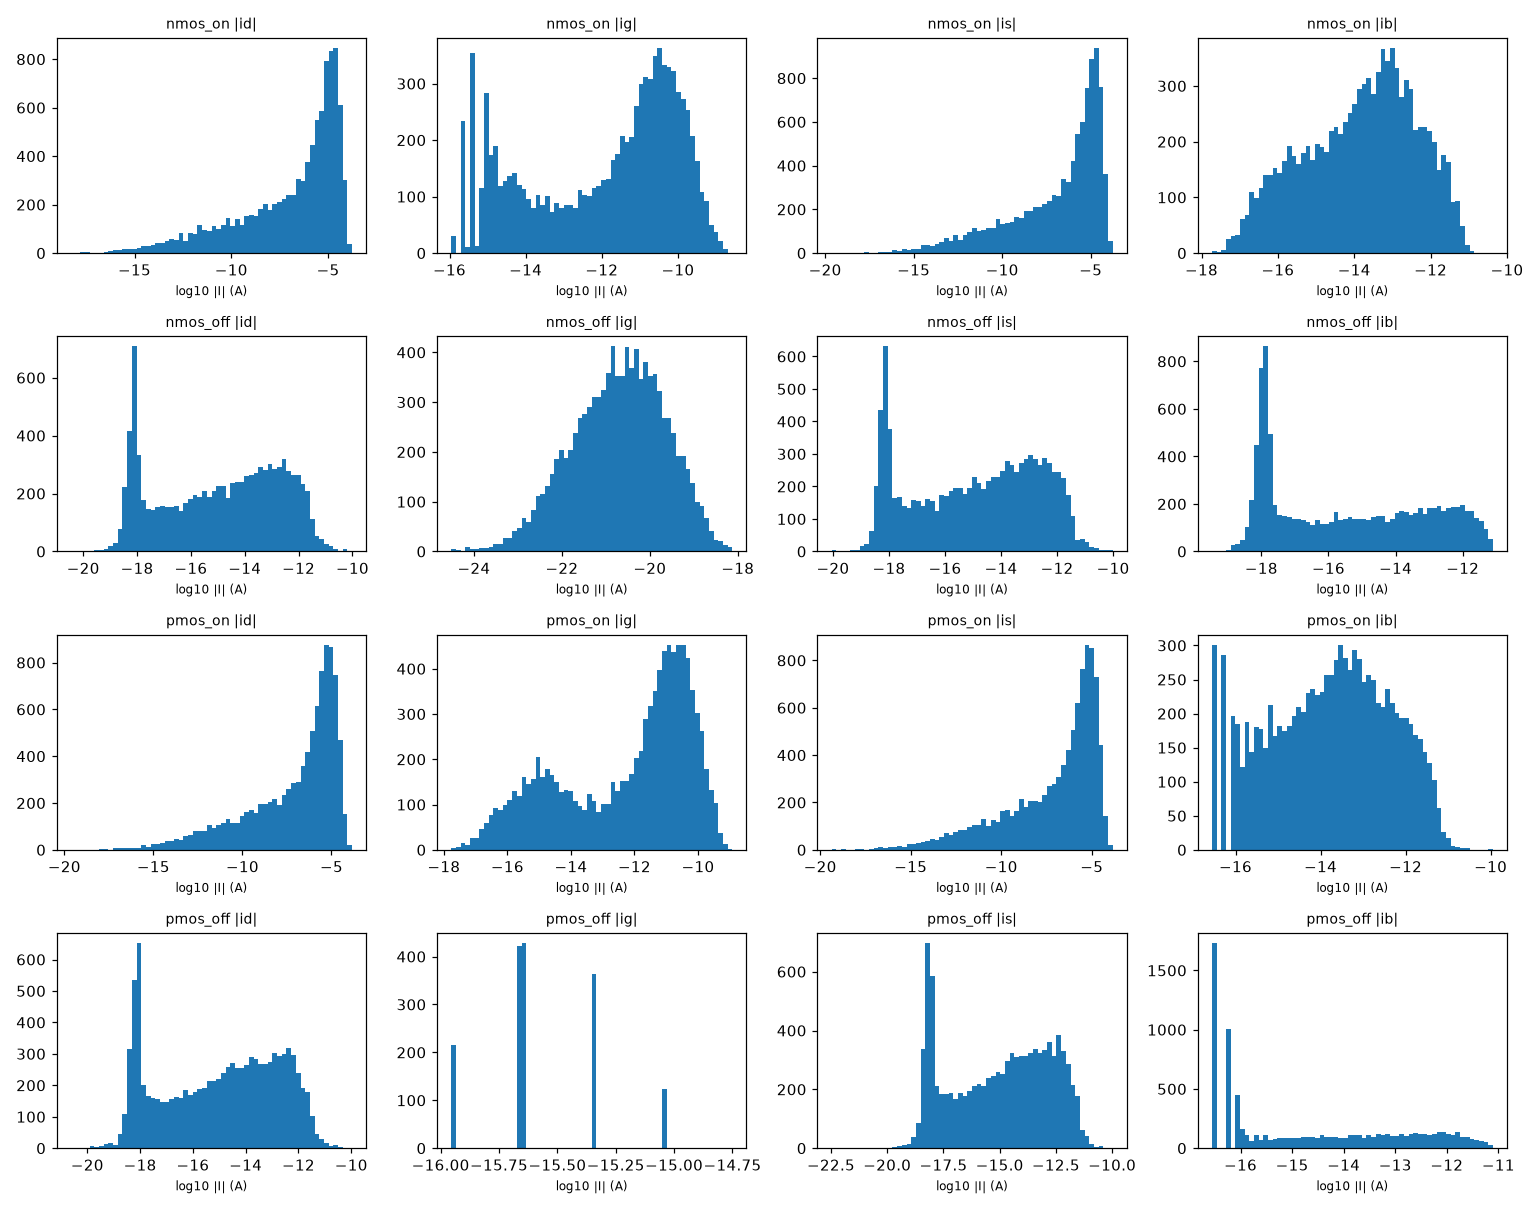
\includegraphics[width=0.95\textwidth]{distributions.png}
\caption{Magnitude distributions of the four terminal currents for the four cases (10{,}000 rows each).}\label{fig:dist}
\end{figure}

\paragraph{Trend plots.} \Cref{fig:trends} shows the three required trends. They come from controlled one-at-a-time SPICE sweeps (all other inputs at
nominal) built with the same netlist generator. All three follow the physically expected direction (\cref{tab:trends}): the OFF current grows by a
factor of about 400 from $-40$ to $125\,^\circ$C (sub-threshold conduction), falls by a factor of 35--46 when $|V_{th0}|$ rises from $-10\,\%$ to
$+10\,\%$, and the gate (oxide-tunnelling) current of an ON device falls by a factor of about 30 when \texttt{toxe} grows from $-10\,\%$ to $+10\,\%$.
\begin{table}[H]
\centering
{\small
\begin{adjustbox}{max width=\linewidth}
\begin{tabular}{llrll}
\toprule
case & expected trend & ratio & sweep end points & check \\
\midrule
NMOS OFF & OFF $I_d$ increases with temperature & 415.3 & 125C / -40C & pass \\
PMOS OFF & OFF $I_d$ increases with temperature & 389.4 & 125C / -40C & pass \\
NMOS OFF & OFF $I_d$ decreases as vth0 increases & 45.61 & |vth0| -10\% / +10\% & pass \\
PMOS OFF & OFF $I_d$ decreases as vth0 increases & 34.82 & |vth0| -10\% / +10\% & pass \\
NMOS ON & ON $I_g$ decreases as toxe increases & 29.57 & toxe -10\% / +10\% & pass \\
PMOS ON & ON $I_g$ decreases as toxe increases & 32.2 & toxe -10\% / +10\% & pass \\
\bottomrule
\end{tabular}
\end{adjustbox}
}
\caption{Automatic checks of the three trend sweeps: expected direction and ratio of the currents at the two ends of each sweep (all other inputs fixed at nominal).}
\label{tab:trends}
\end{table}



\begin{figure}[!htbp]\centering
\begin{subfigure}{0.49\textwidth}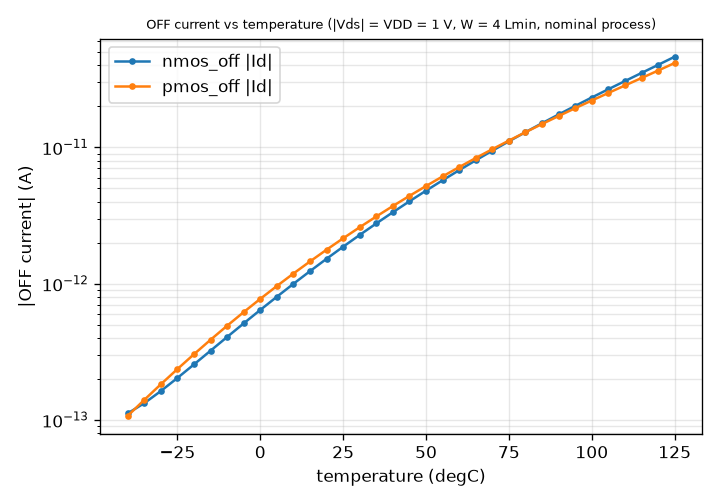
\includegraphics[width=\linewidth]{trend_off_vs_temperature.png}\caption{OFF current vs temperature}\end{subfigure}
\begin{subfigure}{0.49\textwidth}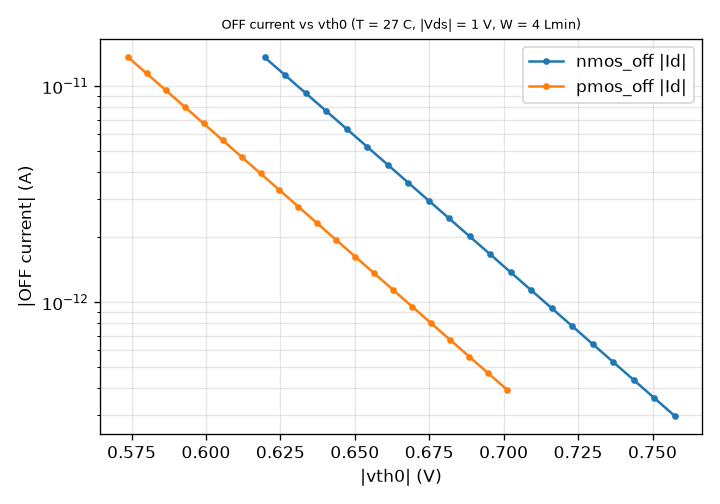
\includegraphics[width=\linewidth]{trend_off_vs_vth0.png}\caption{OFF current vs vth0}\end{subfigure}\\[0.4em]
\begin{subfigure}{0.49\textwidth}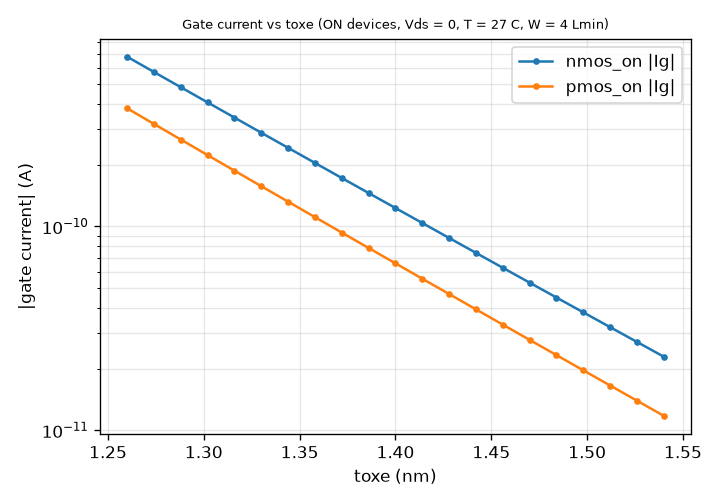
\includegraphics[width=\linewidth]{trend_ig_vs_toxe.png}\caption{Gate current vs toxe (ON devices)}\end{subfigure}
\caption{The three trend plots of the data check.}\label{fig:trends}
\end{figure}
